\chapter*{Author Biography}
\addcontentsline{toc}{chapter}{Author Biography}

\vspace{0.2cm}

\noindent
\begin{minipage}[c]{0.28\textwidth}
    \centering
    \begin{tikzpicture}
        \fill[black!12] (0.04,-0.04) circle (1.4cm);
        \node[circle, draw=rbruGold, line width=2pt, inner sep=0pt] at (0,0) {
            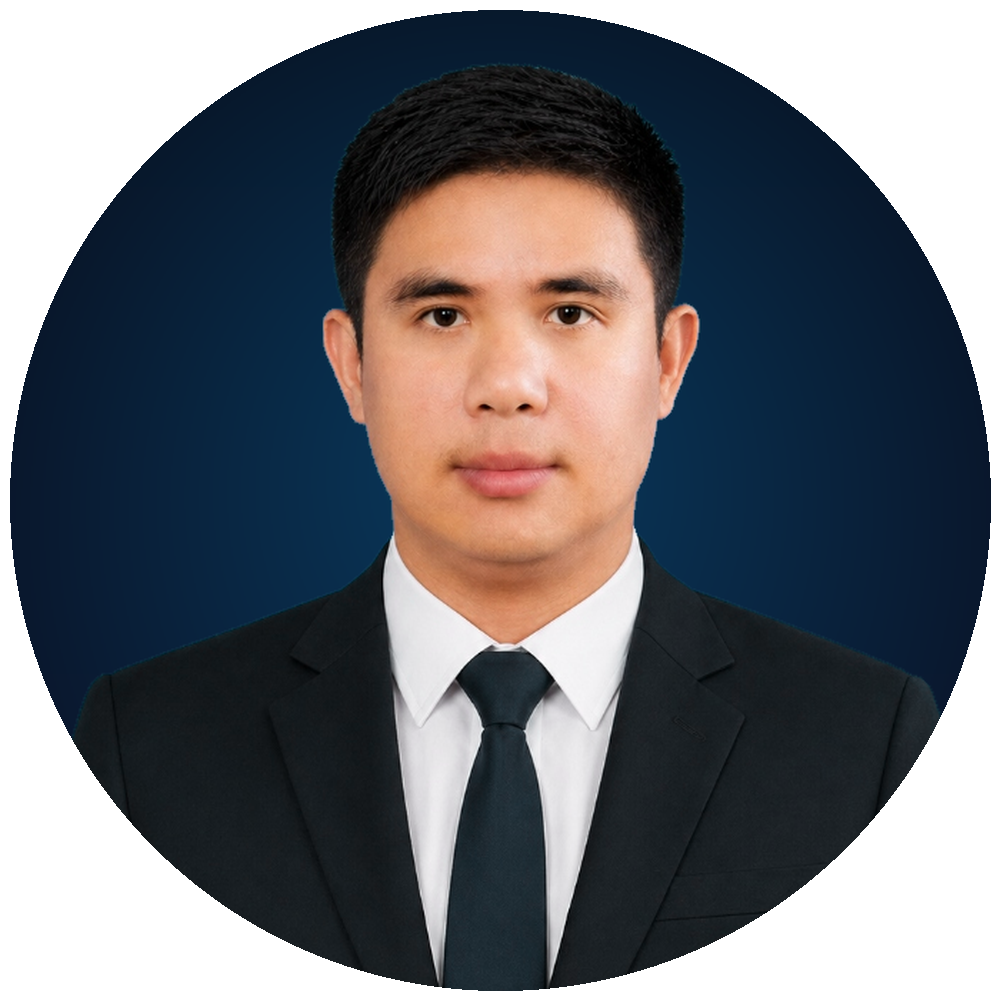
\includegraphics[width=2.7cm,height=2.7cm,keepaspectratio]{images/author_chewa_circle_final.png}
        };
    \end{tikzpicture}
\end{minipage}\hfill
\begin{minipage}[c]{0.69\textwidth}
    {\fontsize{16}{20}\selectfont\bfseries\color{rbruNavy} Asst. Prof. Dr. Chewa Thassana}\\[0.2cm]
    {\fontsize{11.5}{16}\selectfont
    Department of Physics, Faculty of Science and Technology\\
    Rambhai Barni Rajabhat University (RBRU)\\[0.1cm]
    \textbf{Email:} \texttt{chewa.t@rbru.ac.th}}
\end{minipage}

\vspace{0.4cm}
{\color{rbruSlate!30}\hrule height 0.8pt}
\vspace{0.4cm}

\noindent
\begin{minipage}[t]{0.48\textwidth}
    {\fontsize{13}{16}\selectfont\bfseries\color{rbruGreen} Educational Background}\par\vspace{4pt}
    \begin{itemize}\setlength{\itemsep}{2pt}\setlength{\parsep}{0pt}\setlength{\topsep}{2pt}\setlength{\partopsep}{0pt}\setlength{\leftmargin}{12pt}
        \item \textbf{Ph.D. in Physics}\\Doctor of Philosophy in Physics
        \item \textbf{M.Sc. in Physics}\\Master of Science in Physics
        \item \textbf{B.Sc. in Physics}\\Bachelor of Science in Physics (Honors)
    \end{itemize}

    \vspace{0.35cm}
    {\fontsize{13}{16}\selectfont\bfseries\color{rbruGreen} Teaching Responsibilities}\par\vspace{4pt}
    \begin{itemize}\setlength{\itemsep}{2pt}\setlength{\parsep}{0pt}\setlength{\topsep}{2pt}\setlength{\partopsep}{0pt}\setlength{\leftmargin}{12pt}
        \item Mathematics for Physics
        \item Modern Physics \& Quantum Concepts
        \item Advanced Physics Laboratory
        \item Computational Physics \& Scientific Python
    \end{itemize}
\end{minipage}\hfill
\begin{minipage}[t]{0.48\textwidth}
    {\fontsize{13}{16}\selectfont\bfseries\color{rbruGreen} Research Interests}\par\vspace{4pt}
    \begin{itemize}\setlength{\itemsep}{3pt}\setlength{\parsep}{0pt}\setlength{\topsep}{2pt}\setlength{\partopsep}{0pt}\setlength{\leftmargin}{12pt}
        \item \textbf{Theoretical \& Mathematical Physics:} Differential geometry, vector calculus, and nonlinear oscillations.
        \item \textbf{Computational Physics:} High-performance scientific numerical simulations and Python modeling.
        \item \textbf{Immersive Educational Technology:} Augmented, Virtual, and Extended Reality (AR/VR/XR) in STEM.
        \item \textbf{Artificial Intelligence in Education:} Machine learning and AI-assisted physics learning environments.
    \end{itemize}
\end{minipage}
